\chapter{Построение низкоразмерных моделей при неоднородных вариациях пространственных полей}\label{ch:ch4}

\todo{2 pages}

\todo{\cite{Elizarev_2021}}

\begin{align}
    \deriv{u}{\check{t}}
    - \frac{\check{\varkappa}}{\varkappa}
    \frac{\beta^2}{\alpha}  \varkappa \deriv[2]{u}{\check{x}} = \frac{q}{\alpha}
\end{align}

\begin{figure}[ht]
    \centerfloat{
        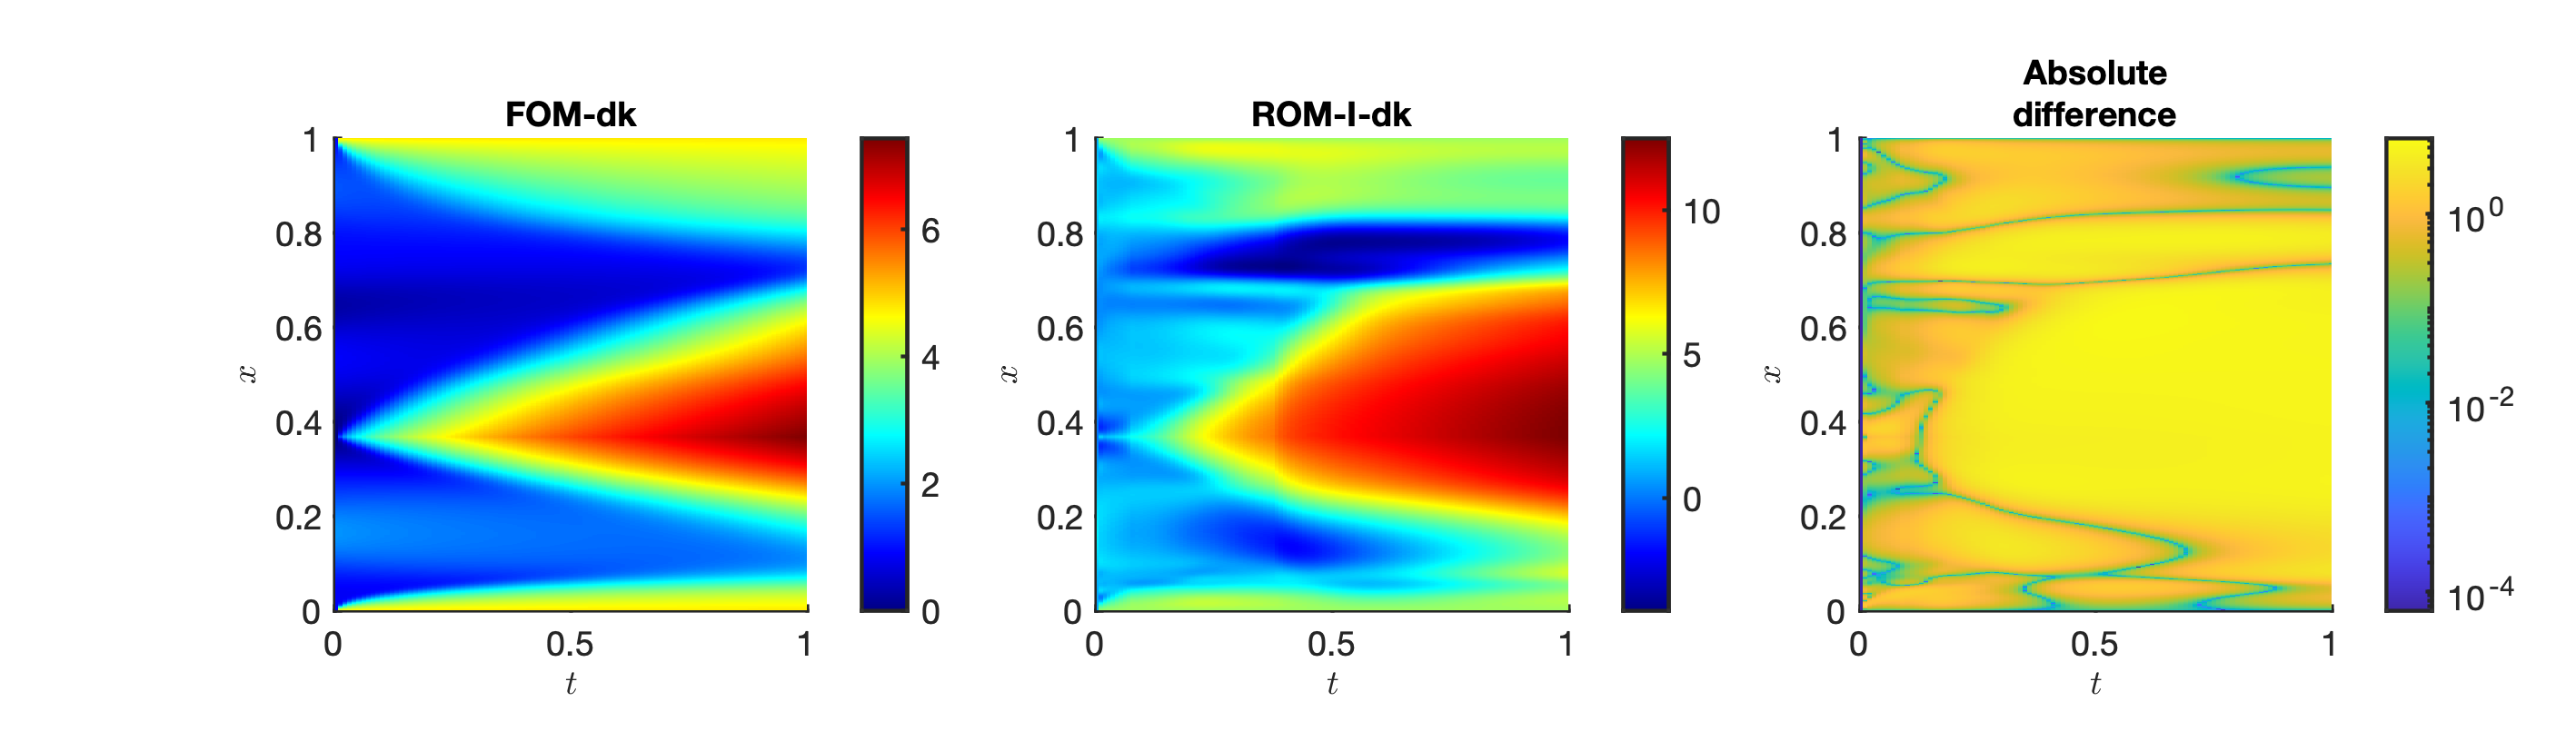
\includegraphics[width=\textwidth,trim={2.5cm 0 0 0},clip]{sci_report/images/ECMOR/11-Problem-K.png}
    }
    \caption{\todo{caption}~\cite{Elizarev2022}}\label{fig:q-domains}
\end{figure}

\begin{figure}[ht]
    \centerfloat{
        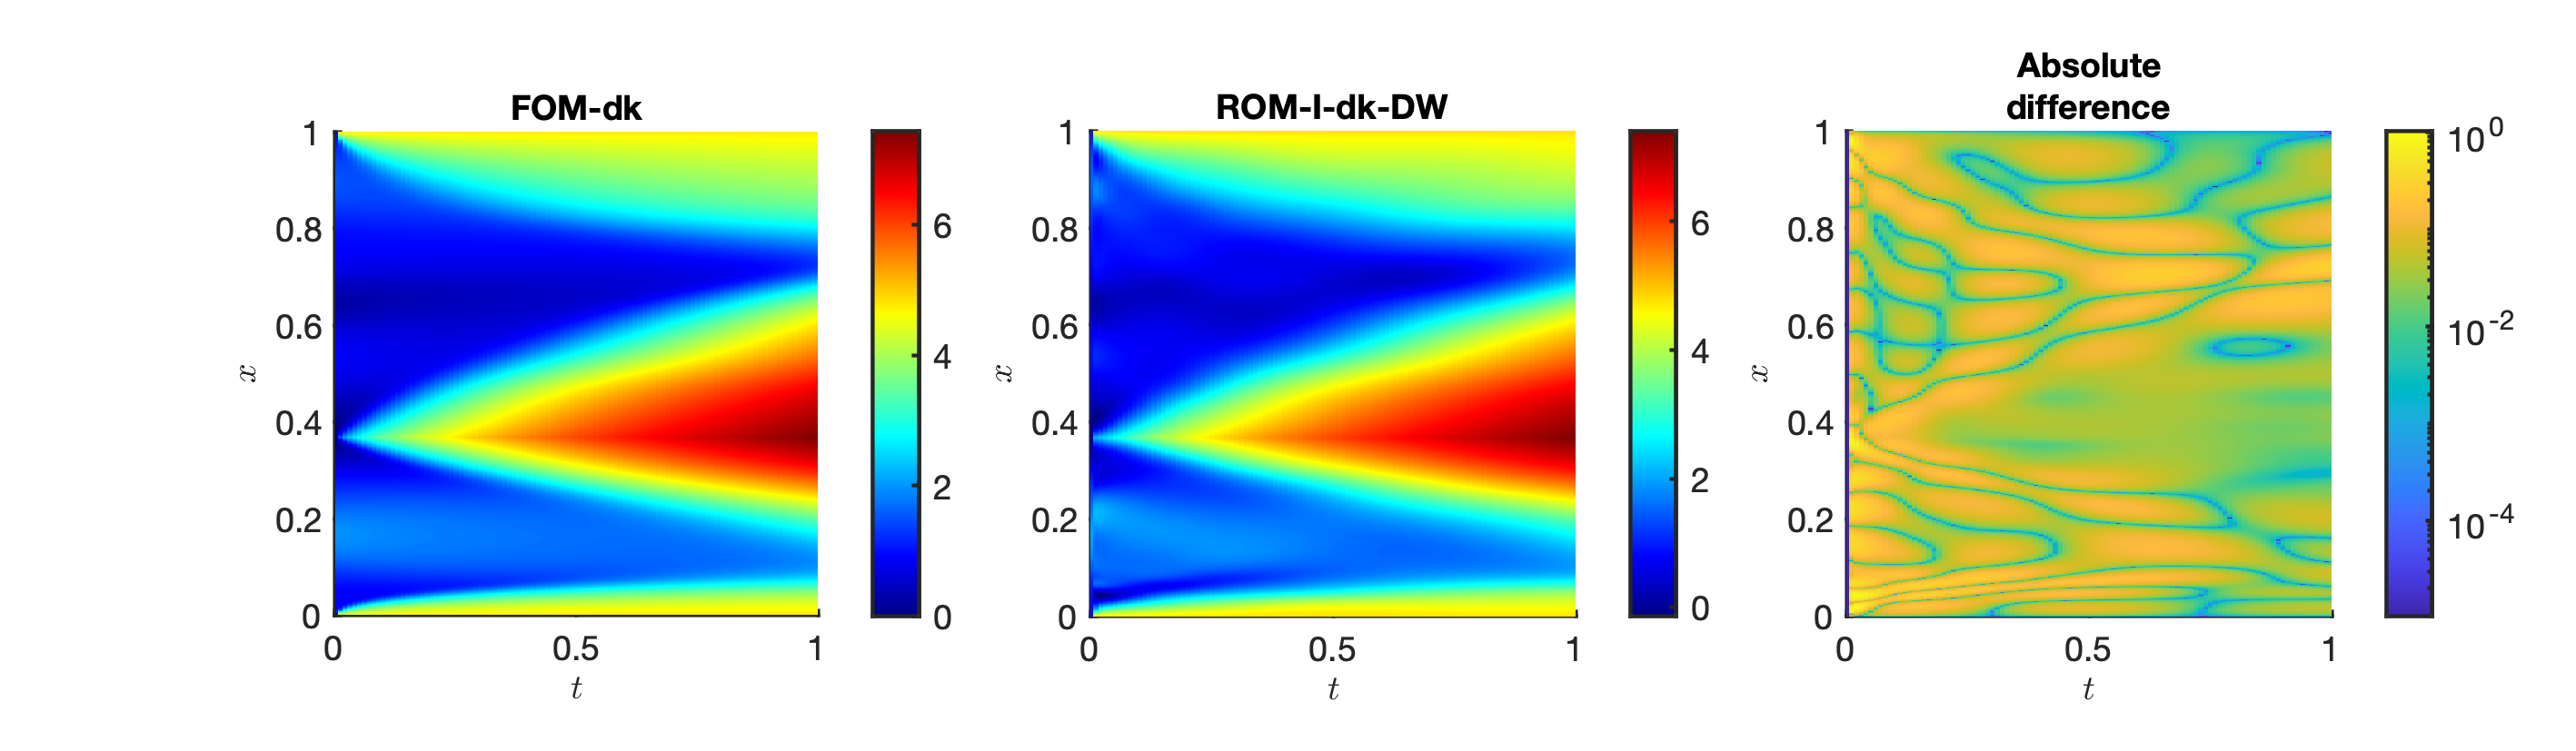
\includegraphics[width=\textwidth,trim={2.5cm 0 0 0},clip]{sci_report/images/ECMOR/15-Result-K.png}
    }
    \caption{\todo{caption}~\cite{Elizarev2022}}\label{fig:q-domains}
\end{figure}
